\subsection{Nutzung von Sonnenenergie}

	\subsubsection{Gegenwärtige Energiequellen}
		Deutschland hat einen Anteil von 38,5\% an regenerativen Energiequellen. Der Anteil an Solarenergie ist über Europa hinweg stark schwankend, der höchste Anteil liegt im Skandinavischen Raum. Die erste Solarzelle wurde 1954 entwickelt und hatte einen Wirkungsgrade zwischen 4 und 6 Prozent.
		\paragraph{Vorteile von Solarzellen}
		\begin{itemize}
			\item Unbegrenzt vorhanden
			\item Emissionslos
			\item Reduzierung von energiepolitischen Abhängigkeiten
		\end{itemize}
		\paragraph{Nachteile von Solarzellen}
		\begin{itemize}
			\item Nicht konstant (Wetter, Jahreszeiten, Tageszeiten...)	
			\item Herstellung nicht emissionsfrei
			\item Hohe Kosten	
		\end{itemize}
	\subsubsection{Brandenburg ist toll}
	\subsubsection{Mögliche Entwicklungen}
		{\bfseries Auslaufzeit der Fossilen Energieträger}
		\begin{itemize}
			\item Kohle ca. 100 Jahre
			\item Erdgas und Erdöl ca. 50 Jahre
			\item Uran ca. 70 Jahre
		\end{itemize}

\subsection{Funktionsweise einer Solarzelle}

	\subsubsection{Grundprinzip}
	
		\paragraph{Massendefekt}
		Nimmt man die Summe aller Nukleonen(Protonen und Neutronen) und vergleicht diese mit der tatsächlich gemessen Masse, so stellt man fest, dass es eine Differenz gibt. Nach Einstein gilt  $E = m\cdot c^2$, also gibt es einen direkten Zusammenhang zwischen Energie und Masse. Der Massendefekt ist somit eine Energiedifferenz, welche die Bindungsenergie. Kommt es nun zu Kernumwandlungen, kann diese Energie freigegeben werden.
		
		\paragraph{Kernfusion}
		Bei der ersten Stufe der Kernfusion in der Sonne kommt es zur einfachen Fusion von einem Deuterium und einem Tritium zu einem Heliumkern und Neutron. Dabei sind Deuterium und Tritium Isotope des Wasserstoffatoms. Sie besitzen einmal 2 (Deuterium) und 3 (Tritium) Neutronen und je ein Proton. Bei der Fusion wird die überschüssige Bindungsenergie in Form von Photonen abgegeben.
		$H^3 + H^2 \rightarrow He + n$
		
		\paragraph{Aufbau}
		95\% aller Solarzellen bestehen aus Silizium, in Speziellen Anwendungsfällen werden auch andere Halbleitermaterialien wie GaAs oder Ge verwendet. Grundlegend besteht eine Solarzelle dann aus einem np-Übergang. Dabei muss die n Schicht sehr dünn sein, damit das einfallende Lich an den Übergang gelangen kann.
		
		\paragraph{Photoelektrischer Effekt}
		Der Photoelektrische Effekt beschreibt zwei unterschiedliche Phänomene. Zum einen gibt es den Äußeren Photoelektrischen Effekt. Bei diesem werden Elektronen durch Bestrahlung aus einer Oberfläche gelöst. Dieser Effekt ist aber nicht weiter für die Funktion von Solarzellen wichtig. Der Innere Photoelektrische Effekt hingegen schon. Bei diesem wird ein Halbleiter durch Lichteinstrahlung leitender, da Elektronen durch die Energie der Photonen aus ein höheres Valenzband gehoben werden.
		
		\paragraph{Ablauf}
		Durch die Lichteinstrahlung werden Elektronen-Lochpaare erzeugt. Innerhalb der Solarzelle müssen diese Ladungen nun getrennt werden, bevor sie sich wieder rekombinieren. Durch die Ladungstrennung kommt es zu einer Leerlaufspannung, welche bei Silizium ungefähr 0.5V beträgt und durch die Bandlücke festgelegt ist.  
		\begin{align}
			Stromabgabe = Generation - Rekombination = J = J_{SC} - J_0 \bigg(e^{\frac{qV}{mkT}}-1\bigg)
		\end{align}
		Die Stromabgabe entspricht dabei der Differenz von generiertem Strom und dem Teil, der wieder rekombiniert. Der Rekombinationsteil kann dabei wie ein Diodenstrom betrachtet werden. Der Wert m ist der Idealitätsfaktor. Er ist ein Wert aus dem Intervall $[1,2]$.

		\paragraph{Kennlinie} Die Kennlinie einer Solarzelle (\ref{9_kennlinie}), welche im Grunde einer Photodiode sehr ähnlich ist, ist die wie einer Diode. Bei Lichteinstrahlung verschiebt sich die Kennlinie.
		\begin{figure}[h]
			\centering
			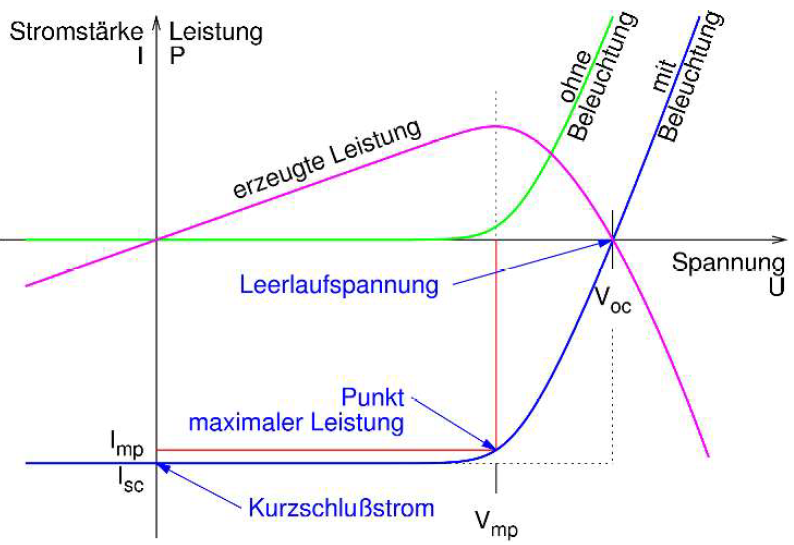
\includegraphics[width=0.3\textwidth]{Kapitel/Kap09/kennlinie.png}
			\caption{Kennlinie einer Solarzelle}
			\label{9_kennlinie}
		\end{figure}
		
		\paragraph{MPP} Innerhalb der Kennlinie kann man den Maximum Power Point (MPP) finden. Die Leistung P berechnet sich wie bekannt durch P = V*J. Der MPP liegt somit kurz hinter dem Knick in der direkten Kennlinie. 
		
		\paragraph{Füllfaktor} Über diesen lässt sich der Füllfaktor bestimmen. Dieser ist das Verhältnis zwischen dem Produkt der Leerlaufspannung und des Kurzschlussstroms und maximaler Leistung:
		\begin{align}
			FF = \frac{P_{max}}{J_{Kurzschluss}V_{Leerlauf}}
		\end{align} 
		Je kleiner der Idealitätsfaktor ist, desto größer ist auch der Füllfaktor.

	\subsubsection{Warum braucht man eine pn-Struktur}

		Der pn-Übergang ist für die Kontaktierung. Die Fermi-Level der Metallkontakte richtet sich nach dem der angrenzenden Majoritäten. Durch den pn-Übergang entsteht ein elektrisches Feld, welches die Ladungen separiert und nach außen trägt. 

	\subsubsection{Wirkungsgrade, Ursachen für Verluste}
	
		\paragraph{Wirkungsgrad} Möchte man nun den Wirkungsgrad berechnen, so benötigt man den MPP und die einfallende Lichtintensität. Der Wirkungsgrad lässt sich somit wie folgt berechnen:\\
		$\eta = \frac{MPP}{Lichtintensität}$
		
		\paragraph{Ursachen für Verluste} Es gibt mehrere Ursachen für Verlust. Zum einen entstehen massive Verluste durch die Unterschiedlichen Wellenlängen des eintretenden Lichts. Ist die Wellenlänge zu groß, so reicht die Energie nicht aus um ein Elektron in das Leitungsband zu heben ($E_g>hf$). Anders herum tritt es auch auf, dass das Licht eine zu niedrige Wellenlänge ausweist. Dann wird ein Elektron auf das höhere Niveau gehoben, die überschüssige Energie wird jedoch in Wärme umgesetzt ($hv > E_g$). Dieses Verhalten lässt sich auch gut durch eine spektrale Darstellung zeigen (\ref{9_spektrum}). Die Verluste können allerdings auch durch den Aufbau aufkommen. So versperren die Kontaktierungen einen Bereich, sodass in diesem kein Licht mehr eintreffen kann. Außerdem gibt es sowohl im Halbleiter, als auch auf den Leitern, ohmsche Widerstandsverluste.
		
		\begin{figure}[h]
			\centering
			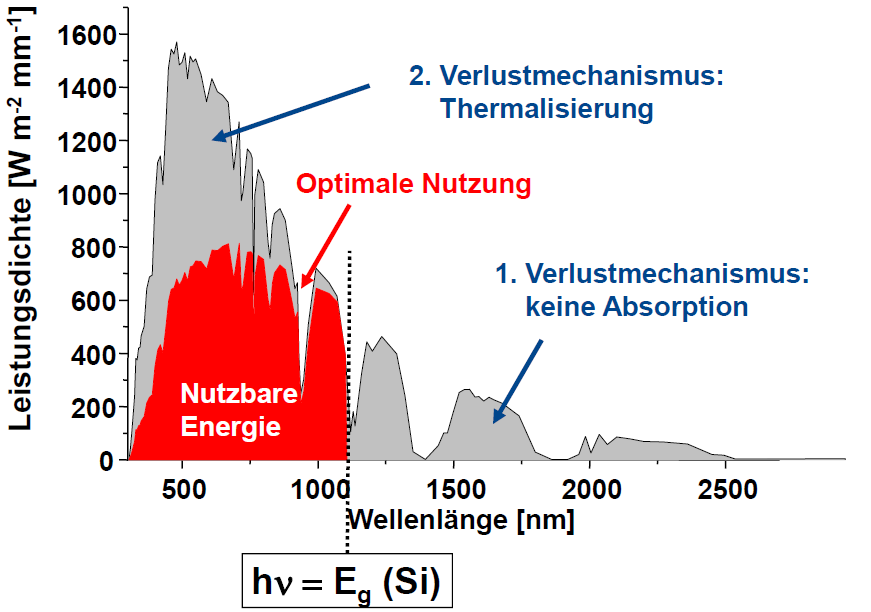
\includegraphics[width=0.6\textwidth]{Kapitel/Kap09/spektrum.png}
			\caption{Spektrale Ausnutzung einer Si-Solarzelle}
			\label{9_spektrum}
		\end{figure}
	

\subsection{Typen von Solarzellen}

	\subsubsection{Verschiedene Materialien}
		\paragraph{Monokristalines Silizium} erreicht Wirkungsgrade von 16-22\%. Somit ist das beste, was aus Silizium hergestellt werden kann. Jedoch ist es sehr teuer.
		
		\paragraph{Polykristalines Silizium} erreicht mit 15-16\% einen recht hohen Wirkungsgrad bei günstigerem Preis.

		\paragraph{Amporphes Silizium} hat einen recht niedrigen Wirkungsgrad mit 6-8\%. Jedoch ist es auch sehr billig und kann für einfache Anwendungen, wie z.B. Taschenrechner o.ä. verwendet werden.

	\subsubsection{Verschiedene Konstruktionen}
		\begin{itemize}
			\item Anschlüsse von hinten, damit weniger Fläche abgedeckt wird
			\item Oberflächentexturierung zur Flächen Maximierung z.B. auf-ätzen
			\item Bündeln mit z.B. Linsen
			\item Mehrere Zellen für verschiedene Wellenlängen hintereinander
		\end{itemize}
		